% future/cpu.tex
% mainfile: ../perfbook.tex
% SPDX-License-Identifier: CC-BY-SA-3.0

\section{The Future of CPU Technology Ain't What it Used to Be}
\label{sec:future:The Future of CPU Technology Ain't What it Used to Be}
%
\epigraph{A great future behind him.}{\emph{David Maraniss}}

과거의 것들은 수많은 해의 경험을 거친 렌즈로 보면 무척 간단하고 순수해
보입니다.
그리고 2000년대 초는 \IX{Moore's Law} 가 그때는 전통적이던 CPU 클락 주파수의
증가를 가져다 주는 것에 대한 임박한 실패로부터 결백했습니다.
오, 기술의 한계에 대한 가끔의 경고가 있긴 했습니다만 그런 경고는 수십년째
들려오고 있었습니다.
그걸 고려하고 다음 시나리오들을 생각해 봅시다:

\iffalse

Years past always seem so simple and innocent when viewed through the
lens of many years of experience.
And the early 2000s were for the most part innocent of the impending
failure of \IX{Moore's Law} to continue delivering the then-traditional
increases in CPU clock frequency.
Oh, there were the occasional warnings about the limits of technology,
but such warnings had been sounded for decades.
With that in mind, consider the following scenarios:

\fi

\begin{figure}[tb]
\centering
\resizebox{3in}{!}{
\includegraphics{cartoons/r-2014-CPU-future-uniprocessor-uber-alles}}
\caption{Uniprocessor \"Uber Alles}
\ContributedBy{Figure}{fig:future:Uniprocessor \"Uber Alles}{Melissa Broussard}
\end{figure}

\begin{figure}[tb]
\centering
\resizebox{2.6in}{!}{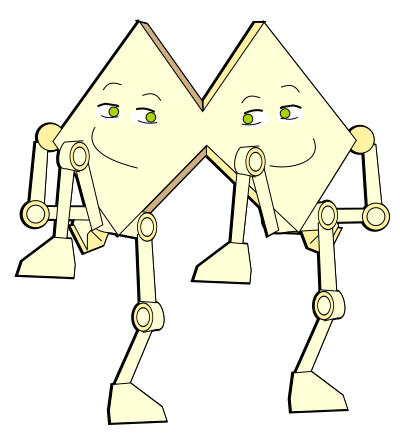
\includegraphics{cartoons/r-2014-CPU-Future-Multithreaded-Mania}}
\caption{Multithreaded Mania}
\ContributedBy{Figure}{fig:future:Multithreaded Mania}{Melissa Broussard}
\end{figure}

\begin{figure}[tb]
\centering
\resizebox{2.5in}{!}{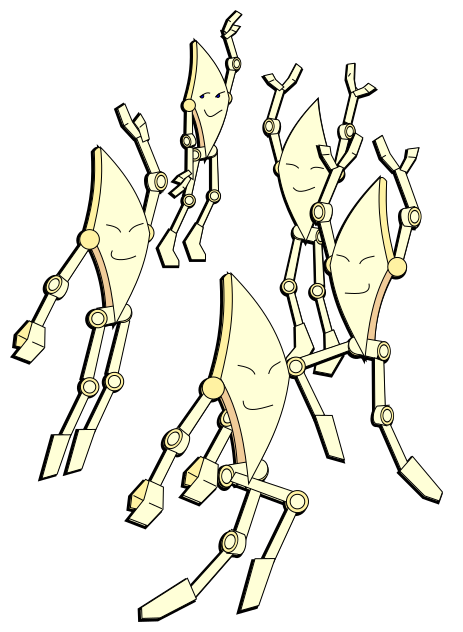
\includegraphics{cartoons/r-2014-CPU-Future-More-of-the-Same}}
\caption{More of the Same}
\ContributedBy{Figure}{fig:future:More of the Same}{Melissa Broussard}
\end{figure}

\begin{figure}[tb]
\centering
\resizebox{3in}{!}{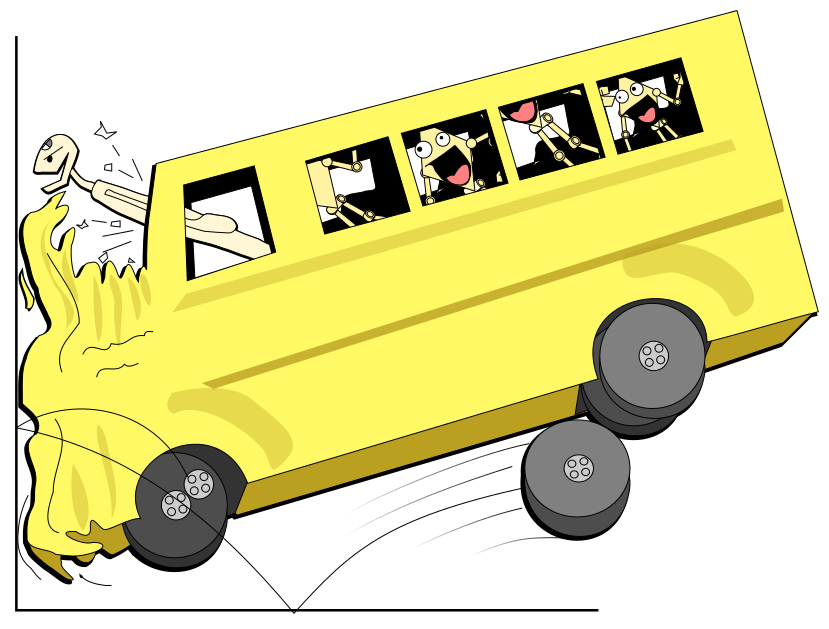
\includegraphics{cartoons/r-2014-CPU-Future-Crash-dummies}}
\caption{Crash Dummies Slamming into the Memory Wall}
\ContributedBy{Figure}{fig:future:Crash Dummies Slamming into the Memory Wall}{Melissa Broussard}
\end{figure}

\begin{figure}[tb]
\centering
\resizebox{3in}{!}{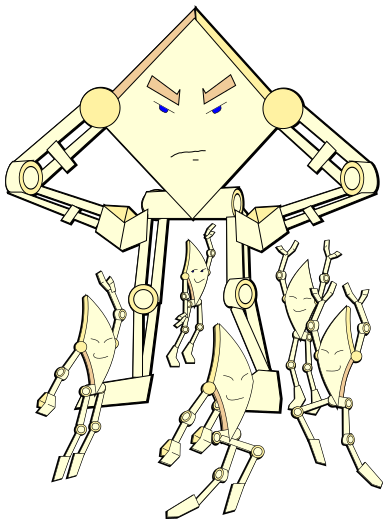
\includegraphics{cartoons/r-2021-CPU-future-astounding-accelerator}}
\caption{Astounding Accelerators}
\ContributedBy{Figure}{fig:future:Astounding Accelerators}{Melissa Broussard, remixed}
\end{figure}

\begin{enumerate}
\item	Uniprocessor \"Uber Alles
	(\Cref{fig:future:Uniprocessor \"Uber Alles}),
\item	Multithreaded Mania
	(\Cref{fig:future:Multithreaded Mania}),
\item	More of the Same
	(\Cref{fig:future:More of the Same}), and
\item	Crash Dummies Slamming into the Memory Wall
	(\Cref{fig:future:Crash Dummies Slamming into the Memory Wall}).
\item	Astounding Accelerators
	(\Cref{fig:future:Astounding Accelerators}).
\end{enumerate}

이 시나리오 각각은 다음 섹션들에서 다루어집니다.

\iffalse

Each of these scenarios is covered in the following sections.

\fi

\subsection{Uniprocessor \"Uber Alles}
\label{sec:future:Uniprocessor \"Uber Alles}

2004년에 다음과 같이 말해진 바와 같이~\cite{PaulEdwardMcKenneyPhD}:

\iffalse

As was said in 2004~\cite{PaulEdwardMcKenneyPhD}:

\fi

\begin{quote}
	이 시나리오에서, \IXalt{Moore's-Law}{Moore's Law} 가 CPU 클락 비율을
	늘려가는 현상과 수평적으로 확장되는 컴퓨팅의 계속된 진보의 결합으로
	인해 SMP 시스템을 무의미하게 만듭니다.
	이 시나리오는 따라서 ``Uniprocessr \"Uber Alles'' 라고 불리게 되는데,
	말 그대로 모든 것들보다도 유니프로세서를 사용하게 되는 시나리오입니다.

	이 유니프로세서 시스템은 인스트럭션 오버헤드만을 겪게 될텐데, 메모리
	배리어, 캐쉬 쓰래싱, 경쟁은 단일 CPU 시스템에 영향을 끼치지 않기
	때문입니다.
	이 시나리오에서, RCU 는 NMI 와의 상호작용 같은 일부 어플리케이션에서만
	유용합니다.
	RCU 를 제공하지 않는 운영체제가 이를 도입할 필요를 겪을지는 명확치
	않은데, 이미 RCU 를 구현한 운영체제는 계속 그럴 수 있긴 합니다.

	그러나, 최근의 멀티쓰레드 CPU 의 발전은 이 시나리오는 실현 가능성이
	상당히 적을 것을 암시하는 것 같습니다.

	\iffalse

	In this scenario, the combination of \IXalt{Moore's-Law}{Moore's Law}
	increases in CPU
	clock rate and continued progress in horizontally scaled computing
	render SMP systems irrelevant.
	This scenario is therefore dubbed ``Uniprocessor \"Uber
	Alles'', literally, uniprocessors above all else.

	These uniprocessor systems would be subject only to instruction
	overhead, since memory barriers, cache thrashing, and contention
	do not affect single-CPU systems.
	In this scenario, RCU is useful only for niche applications, such
	as interacting with NMIs.
	It is not clear that an operating system lacking RCU would see
	the need to adopt it, although operating
	systems that already implement RCU might continue to do so.

	However, recent progress with multithreaded CPUs seems to indicate
	that this scenario is quite unlikely.

	\fi

\end{quote}

실제로 실현가능성이 적습니다!
그러나 더 많은 소프트웨어 커뮤니티가 그들이 병렬성을 받아들여야 한다는 사실을
꺼려했고, 그건 이 커뮤니티가 \IXalt{Moore's-Law}{Moore's Law} 가 제공한 CPU
코어 클락 주파수 증가로 인한 ``공짜 점심'' 이 정말로 끝났음으로 결론짓기
전이었습니다.
잊지 마세요: 믿음은 감정이지, 합리적 기술 사고 과정의 결과가 아닐 수 있습니다!

\iffalse

Unlikely indeed!
But the larger software community was reluctant to accept the fact that
they would need to embrace parallelism, and so it was some time before
this community concluded that the ``free lunch'' of
\IXalt{Moore's-Law}{Moore's Law}-induced
CPU core-clock frequency increases was well and truly finished.
Never forget: belief is an emotion, not necessarily the result of a
rational technical thought process!

\fi

\subsection{Multithreaded Mania}
\label{sec:future:Multithreaded Mania}

역시 2004년으로부터~\cite{PaulEdwardMcKenneyPhD}:

\iffalse

Also from 2004~\cite{PaulEdwardMcKenneyPhD}:

\fi

\begin{quote}
	Uniprocessor \"Uber Alles 의 덜 극단적인 변종은 하드웨어 멀티쓰레딩을
	제공하는 유니프로세서를 갖추는데, 실제로 멀티쓰레딩 제공 CPU 는 많은
	데스크탑과 랩탑 컴퓨터 시스템에서 오늘날의 표준입니다.
	가장 공격적인 멀티쓰레딩 제공 CPU 는 모든 캐쉬 계층을 공유하며, 따라서
	CPU 대 CPU 메모리 응답시간을 제거하고, 그 결과 전통적인 동기화
	메커니즘에서의 성능 제약을 크게 줄입니다.
	그러나, 멀티쓰레딩 제공 CPU 는 여전히 메모리 배리어에 의해 발생하는
	경쟁과 파이프라인 정지로 인한 오버헤드를 일으킬 겁니다.
	더 나아가, 모든 하드웨어 쓰레드가 모든 캐쉬를 공유하므로, 특정 하드웨어
	쓰레드에게 사용 가능한 캐쉬는 동일한 싱글 쓰레드 CPU 에서 가능할 것의
	한 부분에 불과할 텐데, 이는 큰 캐쉬 사용량을 갖는 어플리케이션의 성능을
	하락시킬 겁니다.
	또한 제한된 캐쉬 양이 RCU 기반 알고리즘이 그것의 grace period 에 의한
	추가적 메모리 소모로 인한 성능 문제를 일으킬 가능성도 있습니다.
	이 가능성을 조사하는 건 미래의 일입니다.

	\iffalse

	A less-extreme variant of Uniprocessor \"Uber Alles features
	uniprocessors with hardware multithreading, and in fact
	multithreaded CPUs are now standard for many desktop and laptop
	computer systems.
	The most aggressively multithreaded CPUs share all levels of
	cache hierarchy, thereby eliminating CPU-to-CPU memory latency,
	in turn greatly reducing the performance penalty for traditional
	synchronization mechanisms.
	However, a multithreaded CPU would still incur overhead due to
	contention and to pipeline stalls caused by memory barriers.
	Furthermore, because all hardware threads share all levels
	of cache, the cache available to a given hardware thread is a
	fraction of what it would be on an equivalent single-threaded
	CPU, which can degrade performance for applications with large
	cache footprints.
	There is also some possibility that the restricted amount of cache
	available will cause RCU-based algorithms to incur performance
	penalties due to their grace-period-induced additional memory
	consumption.
	Investigating this possibility is future work.

	\fi

	그러나, 그런 성능 하락을 막기 위해선 여러 멀티 쓰레드 제공 CPU 와 멀티
	CPU 칩들이 최소한 캐쉬의 일부 계층을 하드웨어 쓰레드별로 분리시켜야
	합니다.
	이는 각 하드웨어 쓰레드에게 사용 가능한 캐쉬의 양을 늘릴 것입니다만,
	다시 하드웨어 쓰레드 간에 전달되어야 하는 캐쉬라인들을 위한 메모리
	응답시간 증가를 다시 일으킵니다.

	\iffalse

	However, in order to avoid such performance degradation, a number
	of multithreaded CPUs and multi-CPU chips partition at least
	some of the levels of cache on a per-hardware-thread basis.
	This increases the amount of cache available to each hardware
	thread, but re-introduces memory latency for cachelines that
	are passed from one hardware thread to another.

	\fi

\end{quote}

그리고 우리 모두 이 이야기가 단일 소켓에 끼워진 단일 판 위에 여러개의
멀티쓰레딩 코어들이 올라가고 다양한 수준의 코어당 더 적은 수의 활성 쓰레드 수를
위한 최적화와 함께 어떻게 흘러왔는지 압니다.
그러면 질문은 미래의 공유 메모리 시스템은 항상 단일 소켓에 적합할 것인지가
됩니다.

\iffalse

And we all know how this story has played out, with multiple multi-threaded
cores on a single die plugged into a single socket, with varying degrees
of optimization for lower numbers of active threads per core.
The question then becomes whether or not future shared-memory systems will
always fit into a single socket.

\fi

\subsection{More of the Same}
\label{sec:meas:More of the Same}

또다시 2004년으로부터~\cite{PaulEdwardMcKenneyPhD}:

\iffalse

Again from 2004~\cite{PaulEdwardMcKenneyPhD}:

\fi

\begin{quote}
	더-많은-같은것들 시나리오는 메모리 응답시간 비율이 오늘날의 것과
	대략적으로 비슷하게 유지될 것을 가정합니다.

	이 시나리오는 실제로 변화를 가져오는데, 더 많은 같은 것들을 위해,
	interconnect 성능이 \IXalt{Moore's-Law}{Moore's Law} 로 인한 코어 CPU
	성능의 증가와 함께 증가를 계속해야 하기 때문입니다.
	이 시나리오에서, 파이프라인 중단, 메모리 응답시간, 그리고 경쟁으로 인한
	오버헤드는 심각할 것으로 유지되지만 RCU 는 그것이 오늘날 즐기는 것과
	같은 높은 수준의 적용성을 유지하게 됩니다.

	\iffalse

	The More-of-the-Same scenario assumes that the memory-latency
	ratios will remain roughly where they are today.

	This scenario actually represents a change, since to have more
	of the same, interconnect performance must begin keeping up
	with the \IXalt{Moore's-Law}{Moore's Law} increases in core CPU performance.
	In this scenario, overhead due to pipeline stalls, memory latency,
	and contention remains significant, and RCU retains the high
	level of applicability that it enjoys today.

	\fi

\end{quote}

그리고 이 변화는 \IX{Moore's Law} 가 여전히 제공하고 있는 통합의 여지껏
증가하는 수준의 것입니다.
하지만 더 장기적으로는 어떻게 될까요?
판당 더 많은 CPU?
또는 더 많은 I/O, 캐쉬, 그리고 메모리?

서버는 앞의 전략을 선택한 듯 보이고 칩 위의 임베디드 시스템 (SoC) 은 뒤의 것을
선택해 가고 있는 것으로 보입니다.

\iffalse

And the change has been the ever-increasing levels of integration
that \IX{Moore's Law} is still providing.
But longer term, which will it be?
More CPUs per die?
Or more I/O, cache, and memory?

Servers seem to be choosing the former, while embedded systems on a chip
(SoCs) continue choosing the latter.

\fi

\subsection{Crash Dummies Slamming into the Memory Wall}
\label{sec:future:Crash Dummies Slamming into the Memory Wall}

\begin{figure}[tbp]
\centering
\epsfxsize=3in
\epsfbox{future/latencytrend}
% from Ph.D. thesis: related/latencytrend.eps
\caption{Instructions per Local Memory Reference for Sequent Computers}
\label{fig:future:Instructions per Local Memory Reference for Sequent Computers}
\end{figure}

\begin{figure}[htbp]
\centering
\epsfxsize=3in
\epsfbox{future/be-lb-n4-rf-all}
% from Ph.D. thesis: an/plots/be-lb-n4-rf-all.eps
\caption{Breakevens vs. $r$, $\lambda$ Large, Four CPUs}
\label{fig:future:Breakevens vs. r; lambda Large; Four CPUs}
\end{figure}

\begin{figure}[htbp]
\centering
\epsfxsize=3in
\epsfbox{future/be-lw-n4-rf-all}
% from Ph.D. thesis: an/plots/be-lw-n4-rf-all.eps
\caption{Breakevens vs. $r$, $\lambda$ Small, Four CPUs}
\label{fig:future:Breakevens vs. r; Worst-Case lambda; Four CPUs}
\end{figure}

그리고 2004년으로부터 하나 더 인용합니다~\cite{PaulEdwardMcKenneyPhD}:

\iffalse

And one more quote from 2004~\cite{PaulEdwardMcKenneyPhD}:

\fi

\begin{quote}
	만약
	\cref{fig:future:Instructions per Local Memory Reference for Sequent Computers}
	에 보인 메모리 응답시간 경향이 지속된다면, 메모리 응답시간은 인스트럭션
	수행 오버헤드에 비해 상대적으로 증가하길 계속할 겁니다.
	RCU 를 상당히 사용하는 리눅스와 같은 시스템은
	\cref{fig:future:Breakevens vs. r; lambda Large; Four CPUs} 에 보인
	것처럼 RCU 가 이득이 되는 더 많은 사용처를 찾을겁니다.
	이 그림에서 보여지듯, RCU 가 널리 사용되면 증가하는 메모리 응답시간
	비율이 RCU 에게 다른 동기화 메커니즘 대비 증가하는 장점을 제공합니다.
	대조적으로, RCU 를 적게 사용하는 시스템은
	\cref{fig:future:Breakevens vs. r; Worst-Case lambda; Four CPUs}
	에 보인 것처럼 RCU 의 사용이 비용을 절감할 수 있게끔 더 많은 읽기
	비율을 필요로 할 겁니다.
	이 그림에서 볼 수 있듯, RCU 가 적게 사용된다면 증가하는 메모리 응답시간
	비율은 RCU 를 다른 동기화 메커니즘 대비 단점이 더 많게 만듭니다.
	리눅스는 높은 부하 시에 grace period 당 1,600 개가 넘는 콜백을
	보였으므로, 리눅스는 앞의 카테고리에 속한다고 말해도 안전할 겁니다.

	\iffalse

	If the memory-latency trends shown in
	\cref{fig:future:Instructions per Local Memory Reference for Sequent Computers}
	continue, then memory latency will continue to grow relative
	to instruction-execution overhead.
	Systems such as Linux that have significant use of RCU will find
	additional use of RCU to be profitable, as shown in
	\cref{fig:future:Breakevens vs. r; lambda Large; Four CPUs}.
	As can be seen in this figure, if RCU is heavily used, increasing
	memory-latency ratios give RCU an increasing advantage over other
	synchronization mechanisms.
	In contrast, systems with minor
	use of RCU will require increasingly high degrees of read intensity
	for use of RCU to pay off, as shown in
	\cref{fig:future:Breakevens vs. r; Worst-Case lambda; Four CPUs}.
	As can be seen in this figure, if RCU is lightly used,
	increasing memory-latency ratios
	put RCU at an increasing disadvantage compared to other synchronization
	mechanisms.
	Since Linux has been observed with over 1,600 callbacks per grace
	period under heavy load~\cite{Sarma04c},
	it seems safe to say that Linux falls into the former category.

	\fi

\end{quote}

한편으로, 이 구절은 상당한 업데이트가 있는 워크로드에서는 RCU 가 겪을 수 있는
캐쉬 온도 문제를 예측하지 못했는데, 이는 부분적으로 RCU 가 그런 워크로드에서
정말로 사용될 거라고는 생각되지 않았기 때문입니다.
때문에, sequence locking 이 그렇듯 이런 캐쉬 온도 문제가 심각할 수 있는 경우에
\co{SLAB_TYPESAFE_BY_RCU} 가 사용되게 되었습니다.
다른 한편, 이 구절은 또한 RCU 가 스케쥴링 응답시간 절감이나 보안을 위해서도
사용될 것을 예측하지 못했습니다.

이 책을 위해 생성된 많은 데이터가 8개 소켓, 소켓당 28개 코어, 코어당 두개
하드웨어 쓰레드를 장착해 총 448개 하드웨어 쓰레드를 갖는 시스템에서
수집되었습니다.
유휴 시스템 메모리 응답시간은 1 마이크로세컨드 미만인데, 이는 비슷한 크기의
2004년도 시스템 대비 더 나쁘지 않습니다.
어떤 사람들은 이 응답시간이 x86 CPU 제품군의 상대적으로 강한 메모리 순서 규칙
때문에 마이크로세컨드에 가깝다고 주장합니다만, 그 특정 주장이 받아들여지기
전까진 시간이 좀 더 필요할 겁니다.

\iffalse

On the one hand, this passage failed to anticipate the cache-warmth
issues that RCU can suffer from in workloads with significant update
intensity, in part because it seemed unlikely that RCU would really
be used for such workloads.
In the event, the \co{SLAB_TYPESAFE_BY_RCU} has been pressed into
service in a number of instances where these cache-warmth issues would
otherwise be problematic, as has sequence locking.
On the other hand, this passage also failed to anticipate that
RCU would be used to reduce scheduling latency or for security.

Much of the data generated for this book was collected on an eight-socket
system with 28 cores per socket and two hardware threads per core, for
a total of 448 hardware threads.
The idle-system memory latencies are less than one microsecond, which
are no worse than those of similar-sized systems of the year 2004.
Some claim that these latencies approach a microsecond only because of
the x86 CPU family's relatively strong memory ordering, but it may be
some time before that particular argument is settled.

\fi

\subsection{Astounding Accelerators}
\label{sec:future:Astounding Accelerators}

The potential of hardware accelerators was not quite as clear in 2004
as it is in 2021, so this section has no quote.
However, the November 2020 Top 500 list~\cite{Top500} features a great
many accelerators, so one could argue that this section is a view of
the present rather than of the future.
The same could be said of most of the preceding sections.

Hardware accelerators are being put to many other uses, including
encryption, compression, machine learning.

In short, beware of prognostications, including those in the remainder
of this chapter.
